\documentclass[11pt,oneside,spanish,a4paper]{article}
\usepackage[utf8]{inputenc}
\usepackage[spanish]{babel}
\usepackage[a4paper]{geometry}
\usepackage{graphicx}
\usepackage{fancyhdr}
\usepackage[hyphenbreaks]{breakurl}
\usepackage[hyphens]{url}
\usepackage{hyperref}
\usepackage{listings}
\usepackage{lstlinebgrd}
\usepackage{xcolor}
\usepackage{multicol}
\usepackage{pdfpages}

%%%%%%%%%%%%%%%%%%%%
% Nuevos comandos  %
%%%%%%%%%%%%%%%%%%%%
\newcommand{\HRule}{\rule{\linewidth}{0.5mm}}

\hypersetup{
    pdfcreator={pdfLaTeX},   % creator of the document
    colorlinks=true,       % false: boxed links; true: coloblue links
    linkcolor=blue,          % color of internal links (change box color with linkbordercolor)
    citecolor=blue,        % color of links to bibliography
    filecolor=blue,      % color of file links
    urlcolor=blue           % color of external links
}

\pagestyle{fancy}
\addtolength{\textheight}{2cm}
%\addtolength{\voffset}{-1cm}
%\addtolength{\textwidth}{1cm}

\definecolor{light-gray}{gray}{0.9}

\lstset{
  basicstyle=\ttfamily\color{red},%\footnotesize,%\scriptsize,
  language=tcl,
  breaklines=true,
  otherkeywords={+++},
  numbers=left,
  numberstyle=\scriptsize\color{black}
}

\renewcommand{\lstlistingname}{Código}

\lstset{literate=
  {á}{{\'a}}1 {é}{{\'e}}1 {í}{{\'i}}1 {ó}{{\'o}}1 {ú}{{\'u}}1
  {Á}{{\'A}}1 {É}{{\'E}}1 {Í}{{\'I}}1 {Ó}{{\'O}}1 {Ú}{{\'U}}1
  {à}{{\`a}}1 {è}{{\'e}}1 {ì}{{\`i}}1 {ò}{{\`o}}1 {ù}{{\`u}}1
  {À}{{\`A}}1 {È}{{\'E}}1 {Ì}{{\`I}}1 {Ò}{{\`O}}1 {Ù}{{\`U}}1
  {ä}{{\"a}}1 {ë}{{\"e}}1 {ï}{{\"i}}1 {ö}{{\"o}}1 {ü}{{\"u}}1
  {Ä}{{\"A}}1 {Ë}{{\"E}}1 {Ï}{{\"I}}1 {Ö}{{\"O}}1 {Ü}{{\"U}}1
  {â}{{\^a}}1 {ê}{{\^e}}1 {î}{{\^i}}1 {ô}{{\^o}}1 {û}{{\^u}}1
  {Â}{{\^A}}1 {Ê}{{\^E}}1 {Î}{{\^I}}1 {Ô}{{\^O}}1 {Û}{{\^U}}1
  {œ}{{\oe}}1 {Œ}{{\OE}}1 {æ}{{\ae}}1 {Æ}{{\AE}}1 {ß}{{\ss}}1
  {ç}{{\c c}}1 {Ç}{{\c C}}1 {ø}{{\o}}1 {å}{{\r a}}1 {Å}{{\r A}}1
  {€}{{\EUR}}1 {£}{{\pounds}}1 {"}{{``}}1
}

\begin{document}

%%%%%%%%%%%%%%%%%%%%%%%%%
% Carátula del informe  %
%%%%%%%%%%%%%%%%%%%%%%%%%

\begin{titlepage}
\begin{center}

\textsc{\LARGE Instituto Universitario Aeronáutico}\\[0.5cm]
\textsc{\LARGE Especialización en Sistemas Embebidos}\\[2cm]


\includegraphics[width=0.2\textwidth]{img/logo_f_blanco}~\\[2cm]

\textsc{\Large Entornos Inalámbricos}\\[0.5cm]

\HRule \\[0.4cm]
{ \huge \bfseries Trabajos Prácticos \\[0.4cm] }

\HRule \\[1.5cm]

% Author and supervisor
\begin{minipage}{0.4\textwidth}
\begin{flushleft} \large
\emph{Alumno:}\\
Luis Alberto \textsc{Guanuco}\\
Santiago Nicolás \textsc{Nolasco}\\
Sebastian \textsc{Agüero}\\
Franco \textsc{Bocalon}
\end{flushleft}
\end{minipage}
\begin{minipage}{0.4\textwidth}
\begin{flushright} \large
\emph{Docentes:} \\
Víctor \textsc{Frison}\\
Julio \textsc{Echevarría}\\
José \textsc{Ducloux}
\end{flushright}
\end{minipage}
\vfill
{\large Septiembre 2016}

\end{center}
\end{titlepage}

%\lhead{Luis A. Guanuco}
%\chead{\includegraphics[width=0.02\textwidth]{images/logoUTN}}
%\rhead{Arquitectura Embebidas y Proceso de Tiempo Real}
\section{Introducción}
\label{sec:intro}

Se realizarán ejercitaciones sobre plataformas XBee con el objetivo
de entender los \emph{Entornos Inalámbricos}. Se trabajará con los
modos \emph{AT} y \emph{API} a fin de comprar las ventajas y
desventajas de estos. Estos ejemplos prácticos servirán, además,
alcanzar la resolución del \emph{Trabajo Final}.

\subsection{Módulos XBee S2C}
\label{sec:xbee-mod}

Para el establecimiento de una red basado en los estándares 802.15.4
se plantea como requisito la disponibilidad de módulos que implementen
dicho estándar. En nuestro caso se utilizarán los módulos \emph{XBee
  S2C}\footnote{\burl{http://www.digi.com/support/productdetail?pid=4838}}. Las
principales características de estos dispositivos son:
\begin{itemize}
\item Velocidades de datos
  \begin{itemize}
  \item RF 250 Kbps
  \item Comunicación serial hasta 1 Mbps
  \end{itemize}
\item Alcances
  \begin{itemize}
  \item \textsl{Indoor} 60 metros
  \item \textsl{Outdoor} 1200 metros
  \end{itemize}
\item Potencia de transmisión 3.1 mW (+5 dBm). En modo \textsl{Boost}
  6.3 mW (+8 dBm)
\item Sensibilidad de recepción -100 dBm. EN modo \textsl{Boost} -102
  dBm
\item Banda de frecuencia 2.4 GHz (16 canales)
\item 15 puertos digitales I/O (4 entradas analógicas)
\item Alimentación 2.1V a 3.6V. Consumos:
  \begin{itemize}
  \item En la transmisión 33 mA @ 3.3 VDC. En modo \textsl{Boost}45 mA
  \item En la recepción 28 mA @ 3.3 VDC. En modo \textsl{Boost} 31 mA
  \end{itemize}
\end{itemize}

Los puntos anteriores solo describen las principales características
de los módulos XBee 2SC. Para conocer más en detalle se puede acceder
a la hoja de datos disponible en el sitio web del fabricante
\cite{s2c-ds}.

\subsection{Plataformas adicionales}
\label{sec:plat}

Se utilizará \textsl{hardware} adicional que permita establecer la
comunicación de los módulos XBee con una computadora. Sí bien el
Laboratorio de Sistemas embebidos pone a disposición las plataformas
XBoard\footnote{\burl{http://www.cika.com/soporte/Information/Digi-RF/XBee/}}
se necesita adaptar la comunicación serial del módulo XBee con la la
computadora mediante una puerto USB. Para esto se desarrolló la placa
\emph{XBee-MCP Adapter} (Figura \ref{fig:xb-mcp-adap}). Sobre esta
placa se montarán dos módulos, una es el módulo XBee y el otro es la
placa \emph{MCP2200 Breakout
  Module}\footnote{\burl{http://www.microchip.com/DevelopmentTools/ProductDetails.aspx?PartNO=adm00393}}. Este
último proporciona una comunicación serial USB-UART. 
Además se agregaron dos LEDs conectados a los puertos
\texttt{AD1/DIO1} y \texttt{AD2/DIO2}. Opcionalmente se puede conectar
un potenciómetro al conector \texttt{K1} que se encuentra mapeado al
puerto analógico de la XBee, \texttt{AD0/DIO0}.

\begin{figure}[ht]
  \centering
  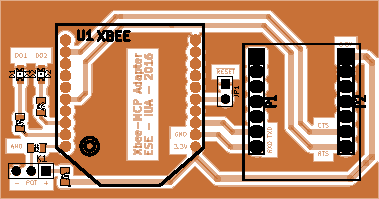
\includegraphics{img/xb-mcp-adapter}
  \caption{Placa XBee-MCP Adapter.}
  \label{fig:xb-mcp-adap}
\end{figure}

La Xboard, anteriormente mencionada, es una plataforma desarrollada
por la empresa Cika Electrónica SRL. La XBoard permite interconectar
los módulos XBee con dispositivos externos \cite{xboard}. En la Figura
\ref{fig:xboard} se presenta una vista superior de la XBoard. Se puede
ver que esta placa tiene un conector hembra con las señales de
comunicación serial, niveles de tensión y otras más. Para conectar la
XBoard a una computadora se utiliza la placa MCP2200 Breakout
Module. Al no requerir componentes externos, se utilizan simplemente
cables que realicen la interconexión de las señales de comunicación
serial.

\begin{figure}[ht]
  \centering
  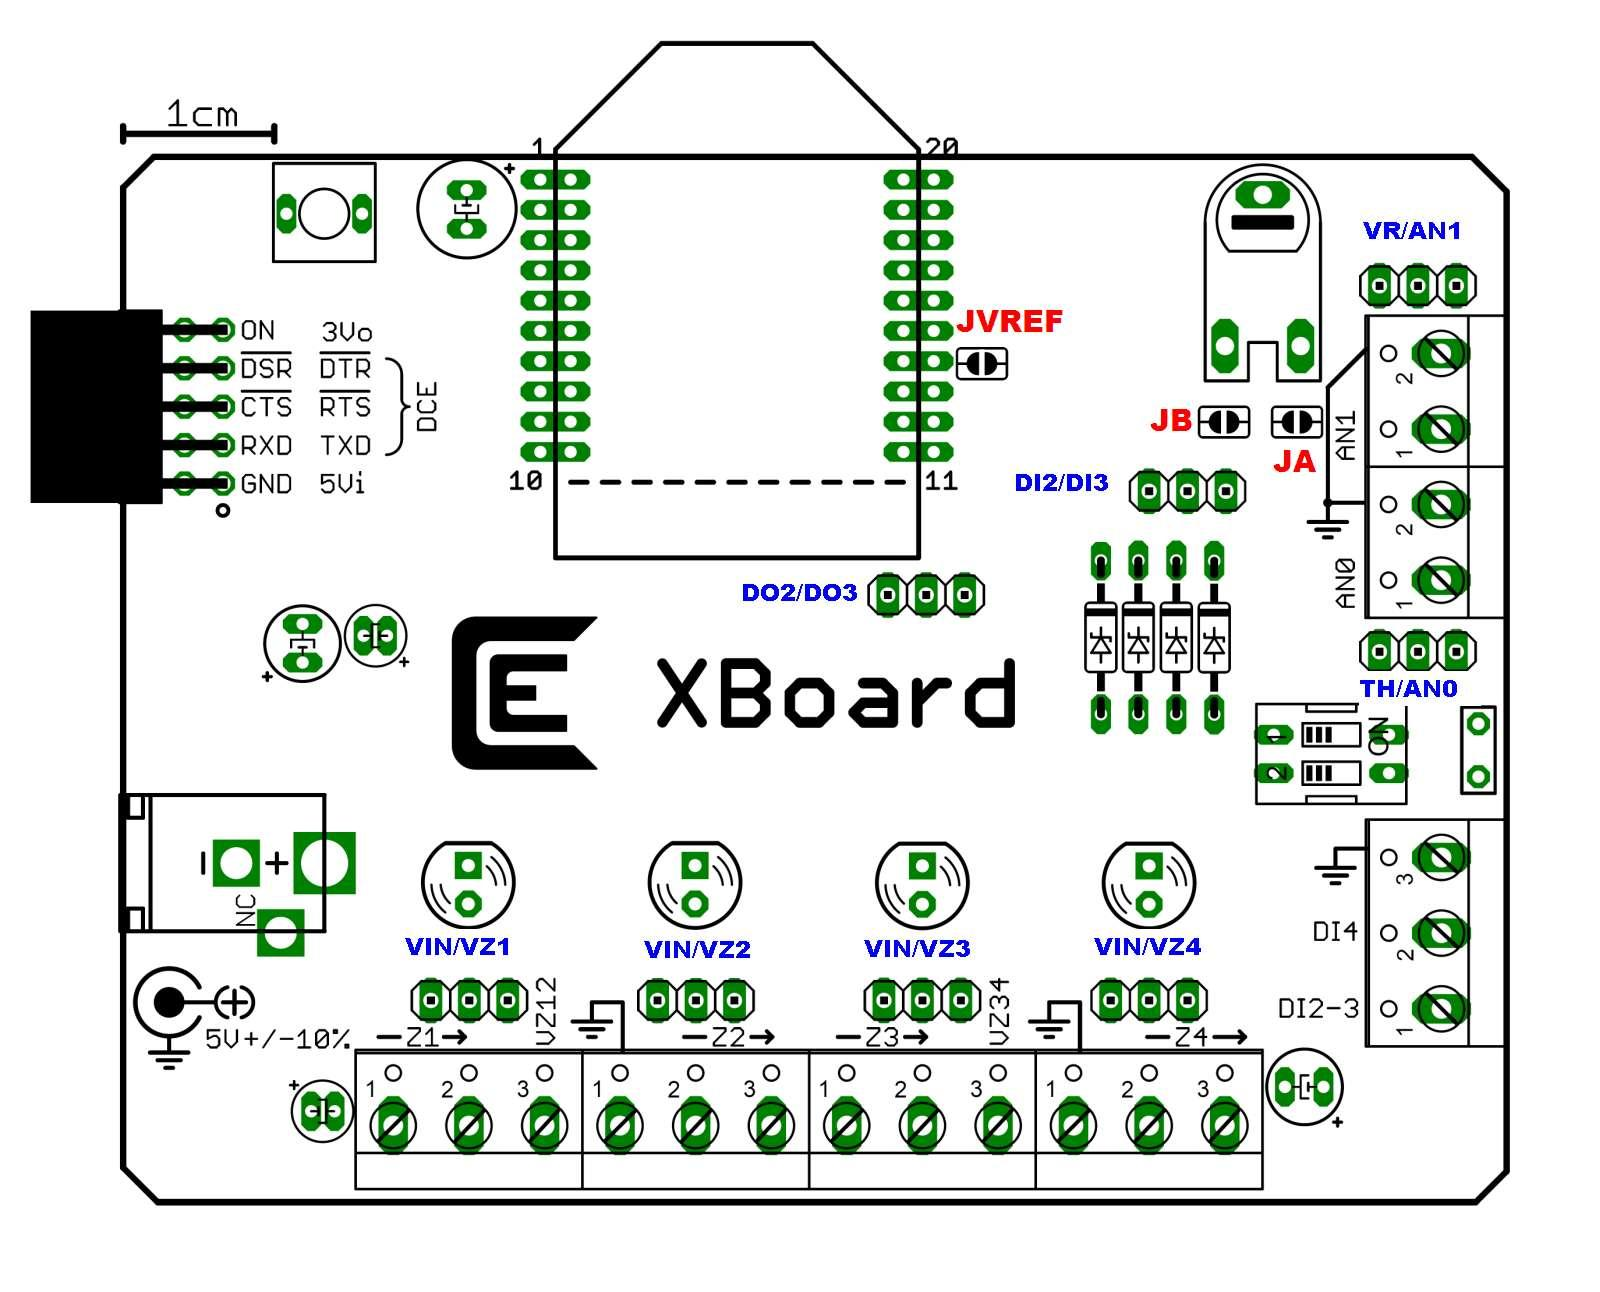
\includegraphics[width=.6\textwidth]{img/xboard}
  \caption{Placa XBoard.}
  \label{fig:xboard}
\end{figure}

Todas las características y configuraciones de las diferentes
plataformas comerciales  se encuentran en la bibliografía referenciada
al final de este documento. 

Se desarrollarán tres tipos de ejercitaciones. La primera sobre los
alcances de RF que proporcionan estos dispositivos. La segunda parte
sobre el manejo de los módulos en modo AT. Y por último se trabajará
en modo API con los módulos sobre una red ZigBee completa. Se
documentarán todos las implementaciones y por último se presentará una
conclusión sobre lo hecho.

\section{Análisis de enlaces}
\label{sec:enlace}

Completar con lo de santiago.

\section{Ejercitación en modo AT}
\label{sec:AT}

El set de comandos AT, también conocidos como set de comandos Hayes,
fue originalmente desarrollado para usar con los modem de Hayes en la
década de 1980. Muchos modems modernos todavía utilizan este
estándar. EL término \emph{comando AT}  viene de usar los caracteres
ASCII para notificar al \textsl{host}  que un le sigue un comando. 

En el caso de los módulos XBee desarrollados por Digi, implementa un
set de comandos propieratrios para interactuar con los módulos de
Digi a través de una comunicación serial. Basado en el set de comandos
AT, Dii usa los caracteres \texttt{AT} antes de cada comando enviado
al modem. Un ejemplo de un comando utilizado por el radio Digi XBee
podría ser \texttt{ATCH}. Este comando es usado para leer o setear el
canal que un radio XBeee es configurado\cite{at-cmds}.

\subsection{Configuración de puertos GPIO}
\label{sec:config-at}

La configuración de los diferentes canales de propósitos generales se
puede realizar utilizando el software XCTU en modo gráfico pero el
objetivo es realizarlo mediante el set de comandos AT. 

\subsubsection{Comando ATIS}
\label{sec:atis}

El comando \texttt{ATIS} fuerza la lectura de todos los canales
habilitados. Analógicos como digitales. En nuestro caso tenemos la
siguiente salida a la petición.

\begin{lstlisting}[emph={+++,ATIS}, emphstyle={\color{blue}}]
+++
OK
ATIS
01
0006
01
0000
0219
\end{lstlisting}

La respuesta que entrega el módulo comienza en la línea \textbf{4}
hasta la \textbf{8}. El primer byte \texttt{01} es la cantidad de
muestra recibidas. En la línea \textbf{5} se tiene configuración de
los canales digitales y la línea \textbf{6} canales analógicos. Para
entender se debe analizar a nivel de bits cada una de las
respuestas. Recuerde que los valores representados están en
hexadecimal. En el primer se tiene $0006_{HEX} =
000000000000110_{BIN}"$ por lo los canales \texttt{DIO1} y
\texttt{DIO2} se encuentran habilitados y configurados como salidas
digitales. Mientras que para los canales analógicos tenemos
$01_{HEX} = 0001_{BIN}$ solo el puerto \texttt{AD0} habilitado. Para
terminar el análisis de la respuesta al comando \texttt{ATIS}, las
líneas \textbf{7} y \textbf{8} son el estado de los canales
digitales y analógicos respectivamente. Como se mencionó
anteriormente, puede visualizarse la configuración de los canales de
I/O en forma gráfica desde el software XCTU. En la Figura
\ref{fig:xctu-setup} se puede ver la misma información que
proporciona el comando \texttt{ATIS}.

\begin{figure}[ht]
  \centering
  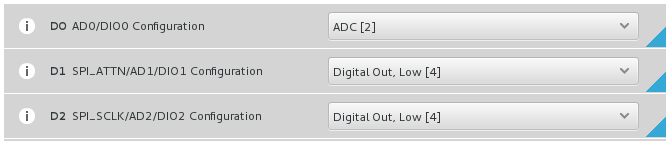
\includegraphics[width=.8\textwidth]{img/xctu-atis}
  \caption{Configuración de los GPIO en modo gráfico.}
  \label{fig:xctu-setup}
\end{figure}

Para dar comienzo con la ejercitación pedida por los docentes, se
deshabilitarán todos los canales de forma tal que el módulo quede sin
ningún GPIO en uso. Sí la configuración es tal como la descrita
anteriormente, se deben aplicar los comandos siguientes.

\noindent\begin{minipage}{.25\textwidth}
\begin{lstlisting}[emph={+++,ATIS,ATD00,ATD10,ATD20,ATWR,ATAC}, emphstyle={\color{blue}}]
+++OK
ATD00
OK
ATD10
OK
ATD20
OK
ATAC
OK
ATWR
OK
ATIS
ERROR
\end{lstlisting}
\end{minipage} \hfill
\begin{minipage}{.70\textwidth}
Para deshabilitar un canal digital/analógico se debe simplemente pasar
como último argumento el valor \texttt{0}. Esto se aplica a los
canales \texttt{DIO0}, \texttt{DIO1} y \texttt{DIO2}. Los comandos que
le siguen son para aplicar los cambios y liberar los \textsl{buffers}
(\texttt{ATAC}) y  escribir la
memoria no-volatil del módulo (\texttt{ATWR}). Al finalizar los
cambios se envía el comando \texttt{ATIS} y se tiene como respuesta
\texttt{ERROR} esto no se debe a un problema de comunicación sino que
al no existir ningún canal habilitado, no puede ofrecer información
alguna. 
\end{minipage}

A continuación se presentan diferentes configuraciones sobre el módulo
XBee montado en la placa XBoard.

\subsubsection{Configurar canales analógicos}

\noindent\begin{minipage}{.35\textwidth}
\begin{lstlisting}[emph={+++,ATIS,ATD02,ATD12,ATWR,ATAC},
    emphstyle={\color{blue}},caption={Canales analógicos.},label=code:2adc]
    +++OK
    ATD02
    OK
    ATD12
    OK
    ATAC
    OK
    ATWR
    OK
    ATIS
    01
    0000
    03
    0268
    0208
\end{lstlisting}  
\end{minipage}\hfill
\begin{minipage}{.60\textwidth}
En el código \ref{code:2adc} se configuran los canales \texttt{DIO0}
y \texttt{DIO1} como analógicos. El último parámetro define este
comportamiento. Luego de guardar la configuración se envía el comando
\texttt{ATIS} para tener la configuración final de todos los
canales. Aquí se puede ver en la línea \textbf{13} no se tiene ningún
canal digital. y en las líneas \textbf{15} y \textbf{16} se ven los
valores de los ADC correspondientes a los canales \texttt{DIO0} y
\texttt{DIO1}.
\end{minipage}

\subsubsection{Configurar canales digitales}
En el caso del código \ref{code:2do} se configuran los canales
\texttt{DIO2} y \texttt{DIO5} como salida. La elección de estos
canales se debe al circuito implementado por la placa XBoard. El
parámetro adicional en los comandos \textbf{3} y \textbf{5} es el
estado digital que se le asignará. El número \texttt{4} aplica un
valor \emph{bajo} mientras que el valor \texttt{5} define un estado
en \emph{alto}.  Al igual que en el caso anterior, el comando
\texttt{ATIS} muestra los estados de los puertos habilitados, en este
caso no tenemos entradas analógicas por lo tanto en la línea
\textbf{14} tenemos 0. 

El código \ref{code:2di}  muestra la configuración de dos canales
digitales de entrada. La diferencia con el caso anterior es el
parámetro asignado. En las líneas \textbf{3} y \textbf{5} el parámetro
es \texttt{3} que configura los canales \texttt{DIO2} y \texttt{DIO4}
como entradas digitales. 

\noindent\begin{minipage}{.45\textwidth}
\begin{lstlisting}[emph={+++,ATIS,ATD25,ATD55,ATWR,ATAC},
    emphstyle={\color{blue}}, caption={Dos salidas
      en alto.}, label=code:2do]
    +++OK
    ATD25
    OK
    ATD55
    OK
    ATAC
    OK
    ATWR
    OK
    ATIS
    01
    0024
    00
    0024
\end{lstlisting}  
\end{minipage}\hfill
\begin{minipage}{.45\textwidth}
\begin{lstlisting}[emph={+++,ATIS,ATD23,ATD43,ATWR,ATAC},
    emphstyle={\color{blue}}, caption={Dos entradas},
 label=code:2di]
    +++OK
    ATD23
    OK
    ATD43
    OK
    ATAC
    OK  
    ATWR
    OK
    ATIS
    01
    0014
    00
    0014
\end{lstlisting}  
\end{minipage}

\subsubsection{Configuración combinada de la XBoard}

\noindent\begin{minipage}{.35\textwidth}
\begin{lstlisting}[emph={+++,ATIS,ATD02,ATD12,ATD25,ATD55,ATD33,ATD43,ATWR,ATAC},
emphstyle={\color{blue}}, caption={GPIO de la placa XBoard.},label=code:completo]
  +++OK
  ATD02
  OK
  ATD12
  OK
  ATD25
  OK
  ATD55
  OK
  ATD33
  OK
  ATD43
  OK
  ATAC
  OK
  ATWR
  OK
  ATIS
  01
  003C
  02
  003C
  0264
\end{lstlisting}  
\end{minipage}\hfill
\begin{minipage}{.60\textwidth}
Finalmente configuraremos la placa XBoard con todos los modos
anteriormente vistos. Los comandos aplicados desde la línea \textbf{2}
hasta la \textbf{12} ya fueron descritos. Como respuesta al comando
\texttt{ATIS} se puede ver todos los canales digitales habilitados
(\texttt{003C}). Mientras que se tiene dos canales analógicos
\texttt{02} y sus respectivos valores en las líneas \textbf{22} y
\textbf{23}.
\end{minipage}
\section{Ejercitación en modo API}
\label{sec:API}
\newpage{}

\section{Enlaces entre módulos XBee}
\label{sec:enlace}

Ya se mostraron en las secciones anteriores las diferentes formas de
manipular los módulos XBee. En esta sección se desarrollarán pruebas
de enlace de los módulos. Las características de radio frecuencia no
son objeto de estudio, se busca evaluar las virtudes en la red que
implementa el estándar 802.15.4. Se utilizará la topología más
sencilla del alcance de las redes Zigbee. Se implementará un
\emph{Coordinador} y los demás serán configurados como
\emph{Dispositivos finales}.




\section{Conclusiones}
\label{sec:conc}

La implementación de este RTOS tan específico y novedoso, por lo menos
para nosotros, nos ha permitido ampliar la concepción de sistemas
operativos en tiempo real. A la vez que se ha podido interactuar con
profesionales de la región que están en pleno desarrollo y aportes
para mejorar el código utilizado (freeOSEK). 

\begin{thebibliography}{1}
\bibitem{s2c-ds}
  Digi International,
  \emph{XBee\textsuperscript{\textregistered{}}/XBee-PRO
    ZigBee\textsuperscript{\textregistered{}} RF Module -- User
    Guide}. 2016.
  
\bibitem{xboard}
  Cika Electrónica SRL.,
  \emph{XBoard [-W]}.
  \burl{http://www.cika.com/soporte/Information/Digi-RF/XBee/XBoard_doc.pdf}.

\bibitem{at-cmds}
  Digi International,
  \emph{Knowledge Base -- The AT Command Set}.
  \burl{http://knowledge.digi.com/articles/Knowledge_Base_Article/The-AT-Command-Set}.

\end{thebibliography}

% \appendix{}

% \chapter{Códigos del programa}
% \label{chap:code-prog}

% \lstinputlisting[basicstyle=\scriptsize,title=Código de la función
% \texttt{main.c}]{src/examples/adc_dac/src/adc_dac.c}

% \lstinputlisting[basicstyle=\scriptsize,title=Código del archivo
% \texttt{proyectofinal.oil}]{src/examples/adc_dac/etc/adc_dac.oil}

% \chapter{Esquemáticos del hardware utulizado}
% \label{chap:sch}

% \includepdf[landscape=true,pages=-]{img/Schematic}

\end{document}
